%! Author = adnansiddiquei
%! Date = 20/12/2023

\subsection{Q5 - Baseline Dataset}\label{subsec:q5}
\subsubsection{Question 5a}\label{subsubsec:q5a}
    \begin{figure}[htb]
    \centering
    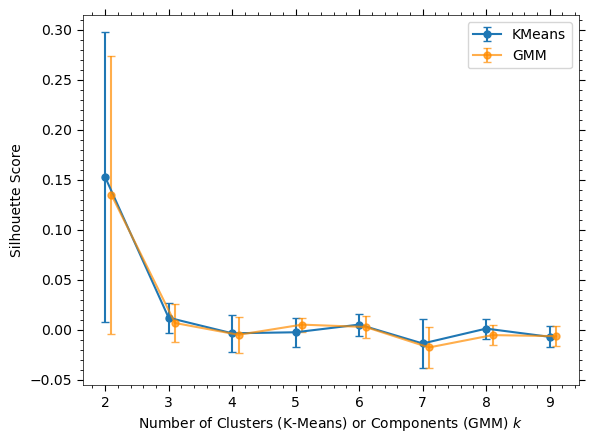
\includegraphics[width=0.9\textwidth]{./figures/q5a_silhouette_scores}
    \caption{The silhouette scores for the K-Means and Gaussian Mixture Models on the pre-processed
        \inlinecode{ADS_baselineDataset.csv} dataset. 5 repetitions were performed to give a mean and standard deviation
        for each $k$ value.}
    \label{fig:q5a_silhouette_scores}
    \end{figure}

    \begin{figure}[htb]
    \centering
    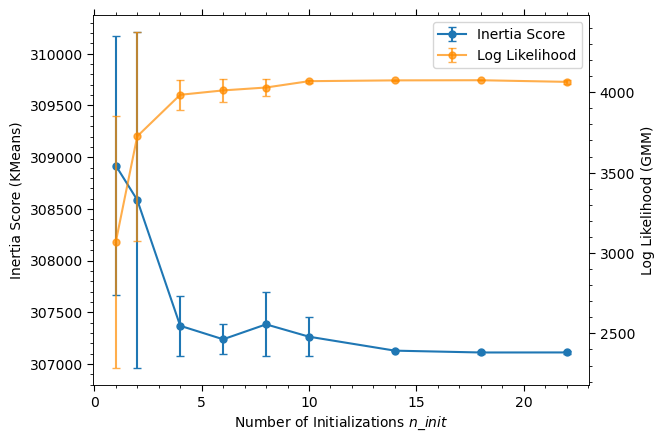
\includegraphics[width=0.9\textwidth]{./figures/q5a_n_init_optimisation}
    \caption{The score of the cost functions for the K-Means and Gaussian Mixture Models as \inlinecode{n_init} is increased
        5 repetitions were performed to give a mean and standard deviation for each \inlinecode{n_init} value.}
    \label{fig:q5a_n_init_optimisation}
    \end{figure}

    \begin{figure}[htb]
    \centering
    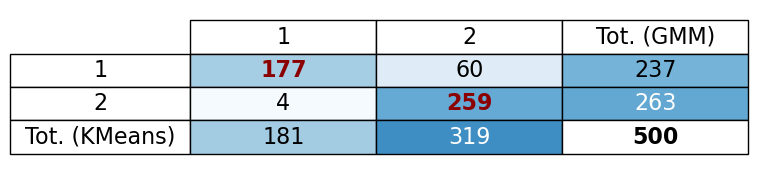
\includegraphics[width=0.9\textwidth]{./figures/q5a_contingency_table}
    \caption{A contingency table comparing cluster assignments for the K-Means and Gaussian Mixture Models on the
        pre-processed \inlinecode{ADS_baselineDataset.csv} dataset, with $k=2$ and $n\_init=50$. The leading diagonal
        gives an 87.2\% agreement between the two models.}
    \label{fig:q5a_contingency_table}
    \end{figure}

    The dataset \inlinecode{ADS_baselineDataset.csv} was pre-processed in the same way as it was for Q4 and Q3e, and
    then K-Means and Gaussian Mixture Models were applied to the dataset.
    The \inlinecode{KMeans} implementation used utilised the Lloyd's algorithm which yields $k$ centroids with each
    sample being assigned to the nearest centroid, this works under the assumption that the data is generally spherically
    distributed.
    The \inlinecode{GaussianMixture} implementation used utilised the expectation-maximisation algorithm which yields $k$
    Gaussian distributions with each sample being assigned to the distribution with the highest probability, this works
    under the assumption that the data is generated by a mixture of Gaussian distributions, so can be a bit more flexible
    than K-Means.

    Fig. \ref{fig:q5a_silhouette_scores} shows the silhouette scores for the K-Means and Gaussian Mixture Models on the
    data, indicating that the optimal number of clusters was $k=2$ for both algorithms.
    However, the large errors on $k=2$ indicated large instability in the algorithms ability to find a global minima,
    as such, Fig. \ref{fig:q5a_n_init_optimisation} shows the effect of increasing the number of initialisations on the
    cost function for both algorithms.
    Both algorithms are very dependent on the random initialisation of the centroids/distributions and the dissappearance
    of the error bars on both models at $n\_init > 10$ indicated that the algorithms required at leeast this many random
    initialisations to find a global minima.
    Therefore, $n\_init=50$ was used hereon.

    Fig. \ref{fig:q5a_contingency_table} shows a contingency table comparing the cluster assignments for the K-Means and
    Gaussian Mixture Models using these parameters, 87.2\% agreement was found.

\subsubsection{Question 5b}\label{subsubsec:q5b}
    \begin{figure}[htb]
    \centering
    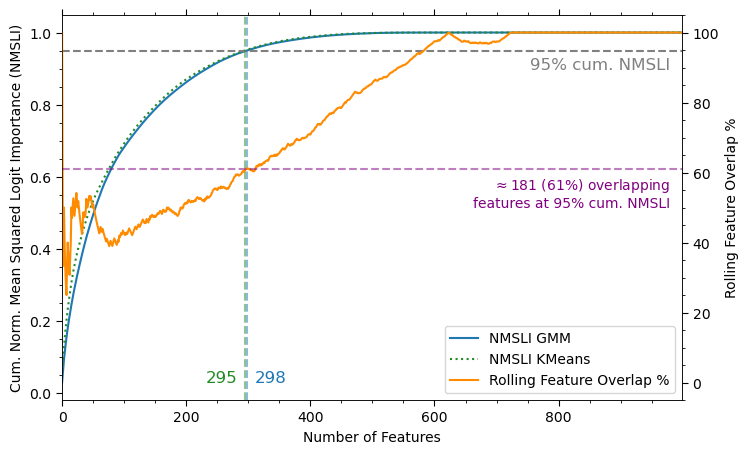
\includegraphics[width=0.9\textwidth]{./figures/q5b_feature_importance}
    \caption{The feature importance for the K-Means and Gaussian Mixture Models using a \inlinecode{LogisticRegression}
        classifier and the NMSLI metric on the classified data shown in Fig. \eqref{fig:q5a_contingency_table}.
        The 95\% NMSLI threshold selected 295 and 298 important features for K-means and GMM respectively, and the
        orange line indicates that roughly 181 of these features were shared between the two models.}
    \label{fig:q5b_feature_importance}
    \end{figure}

    \begin{figure}[htb]
    \centering
    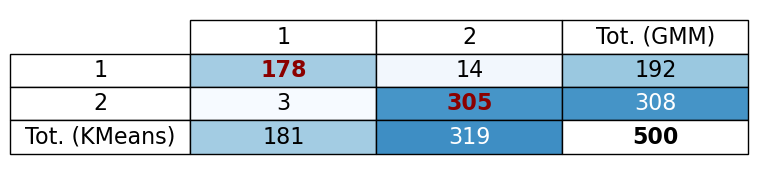
\includegraphics[width=0.9\textwidth]{./figures/q5b_contingency_table}
    \caption{A contingency table comparing cluster assignments for the K-Means and Gaussian Mixture Models after feature
        reduction as shown in Fig. \eqref{fig:q5b_feature_importance}. The leading diagonal shows a 96.6\% agreement
        between the two models.}
    \label{fig:q5b_contingency_table}
    \end{figure}

    A \inlinecode{LogisticRegression} classifier was utilised on the classified data shown in Fig. \eqref{fig:q5a_contingency_table}
    to determine the feature importance, as shown in Fig. \eqref{fig:q5b_feature_importance}, using the NMSLI metric
    (derived and explained in Section \eqref{subsubsec:qf}).
    The top 295 and 298 important features for K-means and GMM respectively were utilised to train a new K-Means and Gaussian
    Mixture Model, as shown in Fig. \eqref{fig:q5b_contingency_table}, 96.6\% agreement was found, a significant improvement
    over the 87.2\% agreement found in Fig. \eqref{fig:q5a_contingency_table}.

\subsubsection{Question 5c}\label{subsubsec:q5c}
    \begin{figure}[htb]
    \centering
    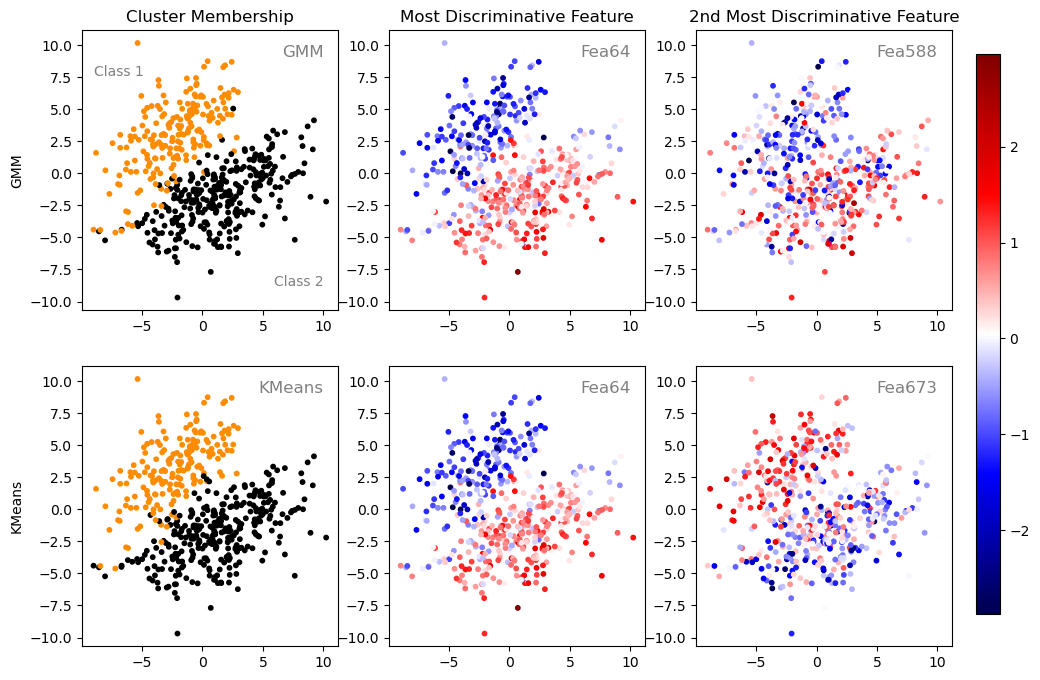
\includegraphics[width=0.9\textwidth]{./figures/q5c}
    \caption{PCA visualisations of the clusters found by the K-Means and Gaussian Mixture Models as shown in Fig.
        \eqref{fig:q5b_contingency_table}. The top row is for the K-Means model and the bottom row is for the GMM.
        The left column shows the cluster membership, the middle and right columns show the samples coloured by the
        first and second most important discriminative respectively. The x-axis is the first principal component and the
        y-axis is the second principal component for all plots.}
    \label{fig:q5c}
    \end{figure}

    Fig. \eqref{fig:q5c} shows the PCA visualisations of the clusters found by the K-Means and Gaussian Mixture Models.
    The middle column indicates a strong positive correlation along $y=-x$ for the most discriminative feature (which was
    the same for both models), and the right column indicates a slightly weaker but still existent positive correlation
    along the same line for the second most discriminative feature (which was different for both models).
